\documentclass{article}
\usepackage[utf8]{inputenc}

\title{CSE 559 HW 2}
\author{Jeremy Schroeter}
\date{April 2024}
\setlength{\parskip}{1em}
\setlength{\parindent}{0em}
\usepackage[margin=1in]{geometry}
\usepackage{amsmath}
\usepackage{amssymb}
\usepackage{mleftright}
\usepackage{amsfonts}
\usepackage{listings}
\usepackage[dvipsnames]{xcolor}
\usepackage{xcolor}
\usepackage{tikz}
\usepackage{titlesec}
\usepackage{enumitem}
\usepackage{graphicx}
\usetikzlibrary{bayesnet}


\begin{document}
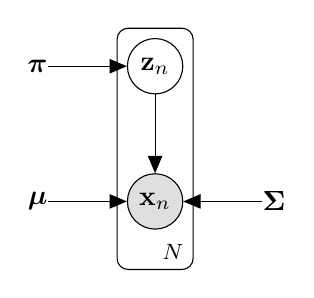
\begin{tikzpicture}

    % Define nodes
    \node[obs]                (x) {$\mathbf{x}_n$};
    \node[latent, above=of x] (z) {$\mathbf{z}_n$};
    \node[const, left=of z] (pi) {$\boldsymbol{\pi}$};
    \node[const, left=of x] (mu) {$\boldsymbol{\mu}$};
    \node[const, right=of x] (sigma) {$\boldsymbol{\Sigma}$};
  
    % Connect the nodes
    \edge {z} {x} ; %
    \edge {pi} {z};
    \edge {mu} {x};
    \edge {sigma} {x};
  
    % Plates
    \plate {xz} {(x)(z)} {$N$} ;
  
  \end{tikzpicture}
\end{document}